\documentclass[11pt]{article}
\usepackage[margin=1in]{geometry}
\usepackage{amsmath,graphicx,booktabs,xcolor,hyperref}
\usepackage[skip=4pt]{caption}
\hypersetup{colorlinks=true,linkcolor=blue!55!black,urlcolor=blue!55!black}
\newcommand{\fig}[1]{\includegraphics[width=\linewidth]{figs/#1}}
\newcommand{\good}[1]{\textcolor{green!45!black}{#1}}
\newcommand{\bad}[1]{\textcolor{red!70!black}{#1}}
\sloppy
\title{\textbf{Why our HCAPO runs started writing essays:}\\[3pt]
\large the length runaway, explained}
\author{Agentic-RL-CA project}
\date{2026-07-30}

\begin{document}
\maketitle

\section*{The short version}
\begin{itemize}
\item We trained a method called \textbf{HCAPO} (``hindsight credit assignment'') on our search-QA
task. In every variant we tried, the model's replies quietly ballooned from about \textbf{90 tokens
to over 1{,}300} per turn --- roughly ten times longer --- while accuracy gained \emph{nothing}
(Figs.~1--2).
\item We first traced it to a genuine \textbf{bug in our port} of the method (we divided by the
wrong thing when computing the hindsight score). We fixed it, verified the fix restored exactly the
behaviour the paper describes --- and then watched the \textbf{fixed version blow up too}, about 40
steps later than the buggy one (Fig.~1, green).
\item The root cause is simple once you see it: HCAPO judges each turn by its \textbf{average
per-token score}, and averages can be gamed by padding. Hard, information-carrying tokens score
low; easy filler scores high; so \emph{a longer, more padded turn looks better than a short, dense
one} (Fig.~3). Training chases that illusion until every turn is maximally padded --- at which point
all turns look alike, the credit signal goes silent (Fig.~4), and the method degenerates into an
expensive version of plain GRPO (Fig.~5).
\item Accuracy never collapsed --- the tokens are \emph{wasted}, not harmful: about \textbf{12$\times$
GRPO's spend for less accuracy}. A deeper diagnostic of the scoring rule is running now; the
candidate fixes are listed at the end.
\end{itemize}

\section{What we saw}
\begin{figure}[h]\centering\fig{fig1_runaway.pdf}
\caption{Average reply length over training for the three HCAPO runs, with plain GRPO (dashed blue)
for scale. All three follow the same script: behave normally for a while, then take off within
$\sim$30 steps and slam into the 2048-token ceiling. Softening the hindsight term ($\omega$=0.5,
orange) only postpones it. Fixing our implementation bug (green) also only postpones it.}
\end{figure}

\begin{figure}[h]\centering\fig{fig2_buy_nothing.pdf}
\caption{The extra words buy nothing. Top: accuracy on our 2{,}048-question validation set ---
flat through the entire explosion, and never better than plain GRPO. Bottom: reply length over the
same steps. If the long replies contained useful extra reasoning or searching, the top panel would
show it. It doesn't.}
\end{figure}

By around step 200 of the fixed run, more than half of all turns were being \emph{cut off} by the
2048-token limit mid-sentence --- the model doesn't ``finish'' its thoughts, it just writes until
the ceiling stops it. Training also got much slower: a step that used to take $\sim$3.5 minutes now
takes $\sim$9, because generating five times the tokens takes five times the time.

\section{Why it happens: averages can be padded}
HCAPO's core idea is reasonable: after an episode ends, re-read each turn \emph{knowing how the
story ended}, and give extra credit to the turns that look pivotal in hindsight. To score ``how
good does this turn look'', it uses the model's own per-token probabilities:
\[
\text{score of a turn} \;=\; \underbrace{\frac{1}{\#\text{tokens}}\sum_{\text{tokens}}
\log p(\text{token})}_{\text{\emph{average} per-token log-probability}}
\qquad\Rightarrow\qquad
\text{credit ratio } \rho \;=\; \frac{\text{this turn's score}}{\text{trajectory average}}
\]
The trouble is the word \emph{average}. The tokens that carry a turn's actual content --- the new
search query, the decision --- are exactly the ones the model finds \emph{hard} (low probability).
The tokens that follow them --- connective tissue, restatements, boilerplate --- are \emph{easy}
(high probability). So the average score of a turn is not a measure of its quality; it is largely a
measure of \textbf{how much easy filler it contains}:

\begin{figure}[h]\centering\fig{fig3_mechanism.pdf}
\caption{Left: a cartoon of the flaw. Two versions of the \emph{same} turn --- one short and dense,
one padded with easy filler. The padded one has a higher \emph{average} score, because averaging
dilutes the hard tokens. Right: the same effect measured in our runs --- in the buggy version the
score climbs straight up with reply length; in the fixed version the mean is pinned at 1 by
construction, so the same pressure shows up in the \emph{spread} instead (Fig.~4).}
\end{figure}

\noindent Once the scorer prefers padded turns, reinforcement learning does the rest: the padded
turns in each batch get a little more credit, the model shifts a little toward padding, and the
cycle repeats. It is an arms race with no winner --- which brings us to the part that surprised us.

\section{We fixed a real bug --- and it wasn't enough}
Our original port computed the credit ratio against the wrong baseline (the turn's ordinary,
non-hindsight probability, instead of the paper's ``average over the trajectory's turns'').
That bug was real and worth fixing: it made the ratio systematically low, half the safety clip
never engaged, and it gave \emph{global} verbosity a direct reward.

The paper's version normalises each turn \emph{against its own trajectory}, so if every turn gets
longer together, the scores cancel and nobody gains. We predicted --- in writing --- that this
would prevent the runaway. \textbf{It did not}, and the reason is instructive: the cancellation
protects against everyone lengthening \emph{in lockstep}, but training never moves in lockstep. In
any given batch, \emph{some} turn is a bit longer and more padded than its siblings, and that turn
wins the comparison. The model is rewarded for being \emph{longer than its own average} --- a
target that moves every time it is chased. Every student on a curved exam still crams; the class
average just keeps rising. The race only ends when every turn is maximally padded and all scores
converge --- and then the signal is gone:

\begin{figure}[h]\centering\fig{fig4_signal_death.pdf}
\caption{The fixed version's runaway consumes its own signal. Green: how much the hindsight scores
actually \emph{differ} between turns (the spread of $\rho$) --- the method's entire information
content. Gray: reply length. As padding homogenises the turns, the spread collapses from 0.135 to
0.030; by step 200 every turn scores $\approx$1.0 and the ``hindsight credit'' distinguishes
nothing. What remains is plain GRPO plus a small position bonus --- at twelve times the price.}
\end{figure}

\section{The bill}
\begin{figure}[h]\centering
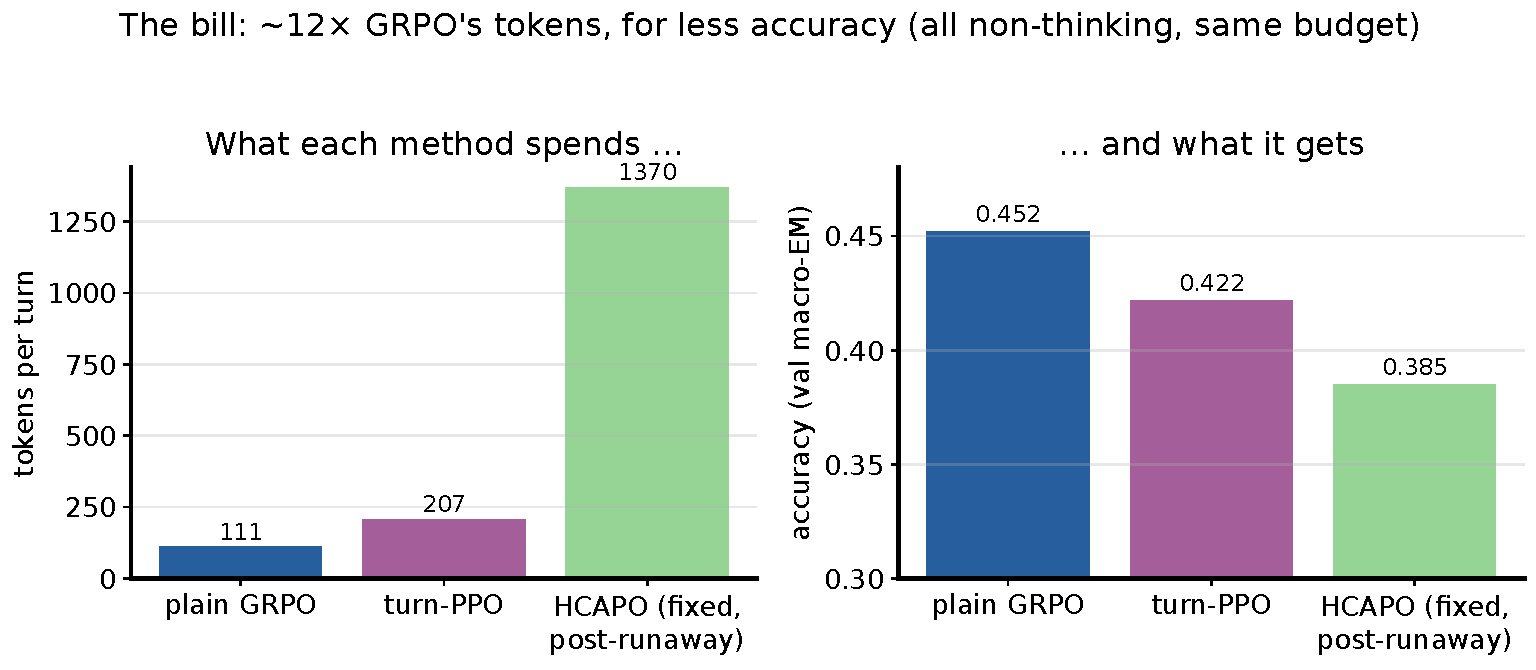
\includegraphics[width=0.9\linewidth]{figs/fig5_cost.pdf}
\caption{Same task, same budget, same non-thinking setup. HCAPO (after its runaway) spends
$\sim$1{,}370 tokens per turn to score \emph{below} both plain GRPO (111 tokens) and turn-PPO
(207 tokens).}
\end{figure}

\section{What we're doing about it}
\textbf{The diagnostic has now run} (456 logged trajectories re-scored under matched conditions:
with the hindsight text, without it, and with the \emph{gold answer} injected instead). Three
findings, each a different nuisance channel:
\begin{itemize}
\item \textbf{The length channel is injected by the hindsight text itself.} Without it, longer
turns do \emph{not} score higher per token (corr $-0.02$ in the healthy regime). Add the hindsight
suffix and a $+0.43$ length correlation appears --- and the ``lift'' (hindsight minus plain score),
which should isolate pure hindsight information, carries \emph{all} of it ($+0.43$ healthy,
$+0.77$ post-runaway, both surviving position controls).
\item \textbf{In the healthy regime, the credit mostly just points at the answer turn.} The
top-credit turn is the \emph{final} (answer) turn in \textbf{73\%} of trajectories --- nearly twice
the 39\% base rate --- because the episode's ending trivially ``explains'' the turn that produced
it. Injecting the gold answer instead of the last retrieval \emph{keeps} this preference: the leak
survives every normalisation we tried.
\item \textbf{The credit's direction flips with the regime.} Healthy: answer turns +0.09 over
search turns, later turns favoured (corr with position $+0.66$). Post-runaway: answer turns
$-0.03$ \emph{under} search turns, earlier turns favoured ($-0.44$) --- the padded search turns
out-score everything. A credit signal whose preferences invert with the policy's own verbosity is
tracking artifacts, not pivotal decisions.
\end{itemize}

\textbf{Candidate fixes, in rough order of appeal:}
\begin{enumerate}
\item \textbf{Stop averaging over a paddable denominator} --- score turns on a fixed window or a
length-controlled statistic, so filler cannot move the score.
\item \textbf{Exclude the final (answer) turn} from hindsight credit --- now measured, not
hypothesised: it is the top-credit turn in 73\% of healthy-regime trajectories, so this changes
most credit assignments.
\item \textbf{Inject the gold answer, not the last retrieval}, as the hindsight context --- shorter,
cleaner, and it cannot reward re-reading your own padding.
\item A blunt \textbf{per-turn length penalty} would mask the symptom, but leaves the mis-scoring in
place --- a last resort, not a fix.
\end{enumerate}

\section*{Fine print}
Single seed per run; all on SearchQA (4-turn episodes, Qwen3-4B, non-thinking, 2048-token cap).
The HCAPO paper's own benchmarks (ALFWorld, WebShop) use short action-style turns under tight
caps, and may simply never enter this regime --- our claim is about this task class, not their
results. Accuracy numbers in Fig.~5 are validation macro-EM; the fixed run is still training and
its final numbers will be appended at step 500. Full technical trail (timestamped pre-registrations,
two retracted over-calls, and the falsified prediction): \texttt{docs/reports/}
\texttt{2026-07-21\_4b\_horizon\_eval/results/hcapo\_wave3\_preregistration.md} and the companion
technical note \texttt{2026-07-29\_hcapo\_implementation\_note/}. Rebuild:
\texttt{assets/build\_figures.py} + \texttt{tectonic report.tex}.
\end{document}
